\chapter{Contexte et cahier des charges}
\section{Présentation des outils à conecter}

\subsection{Relume}

Relume est un outil innovant en SaaS, conçu pour révolutionner la création de sites web grâce à l'intelligence artificielle. Il permet de générer rapidement des plans de site et des wireframes UX, tout en s'intégrant de manière fluide avec Figma et Webflow via un simple processus de copier-coller. L’interface intuitive de Relume embarque les utilisateurs dès l’onboarding, où la description succincte d’un site suffit pour que l’IA crée automatiquement une arborescence complète. Ce processus non seulement économise du temps, mais rend également accessible la création de sites web professionnels.

\begin{figure}[h] 
  \centering
  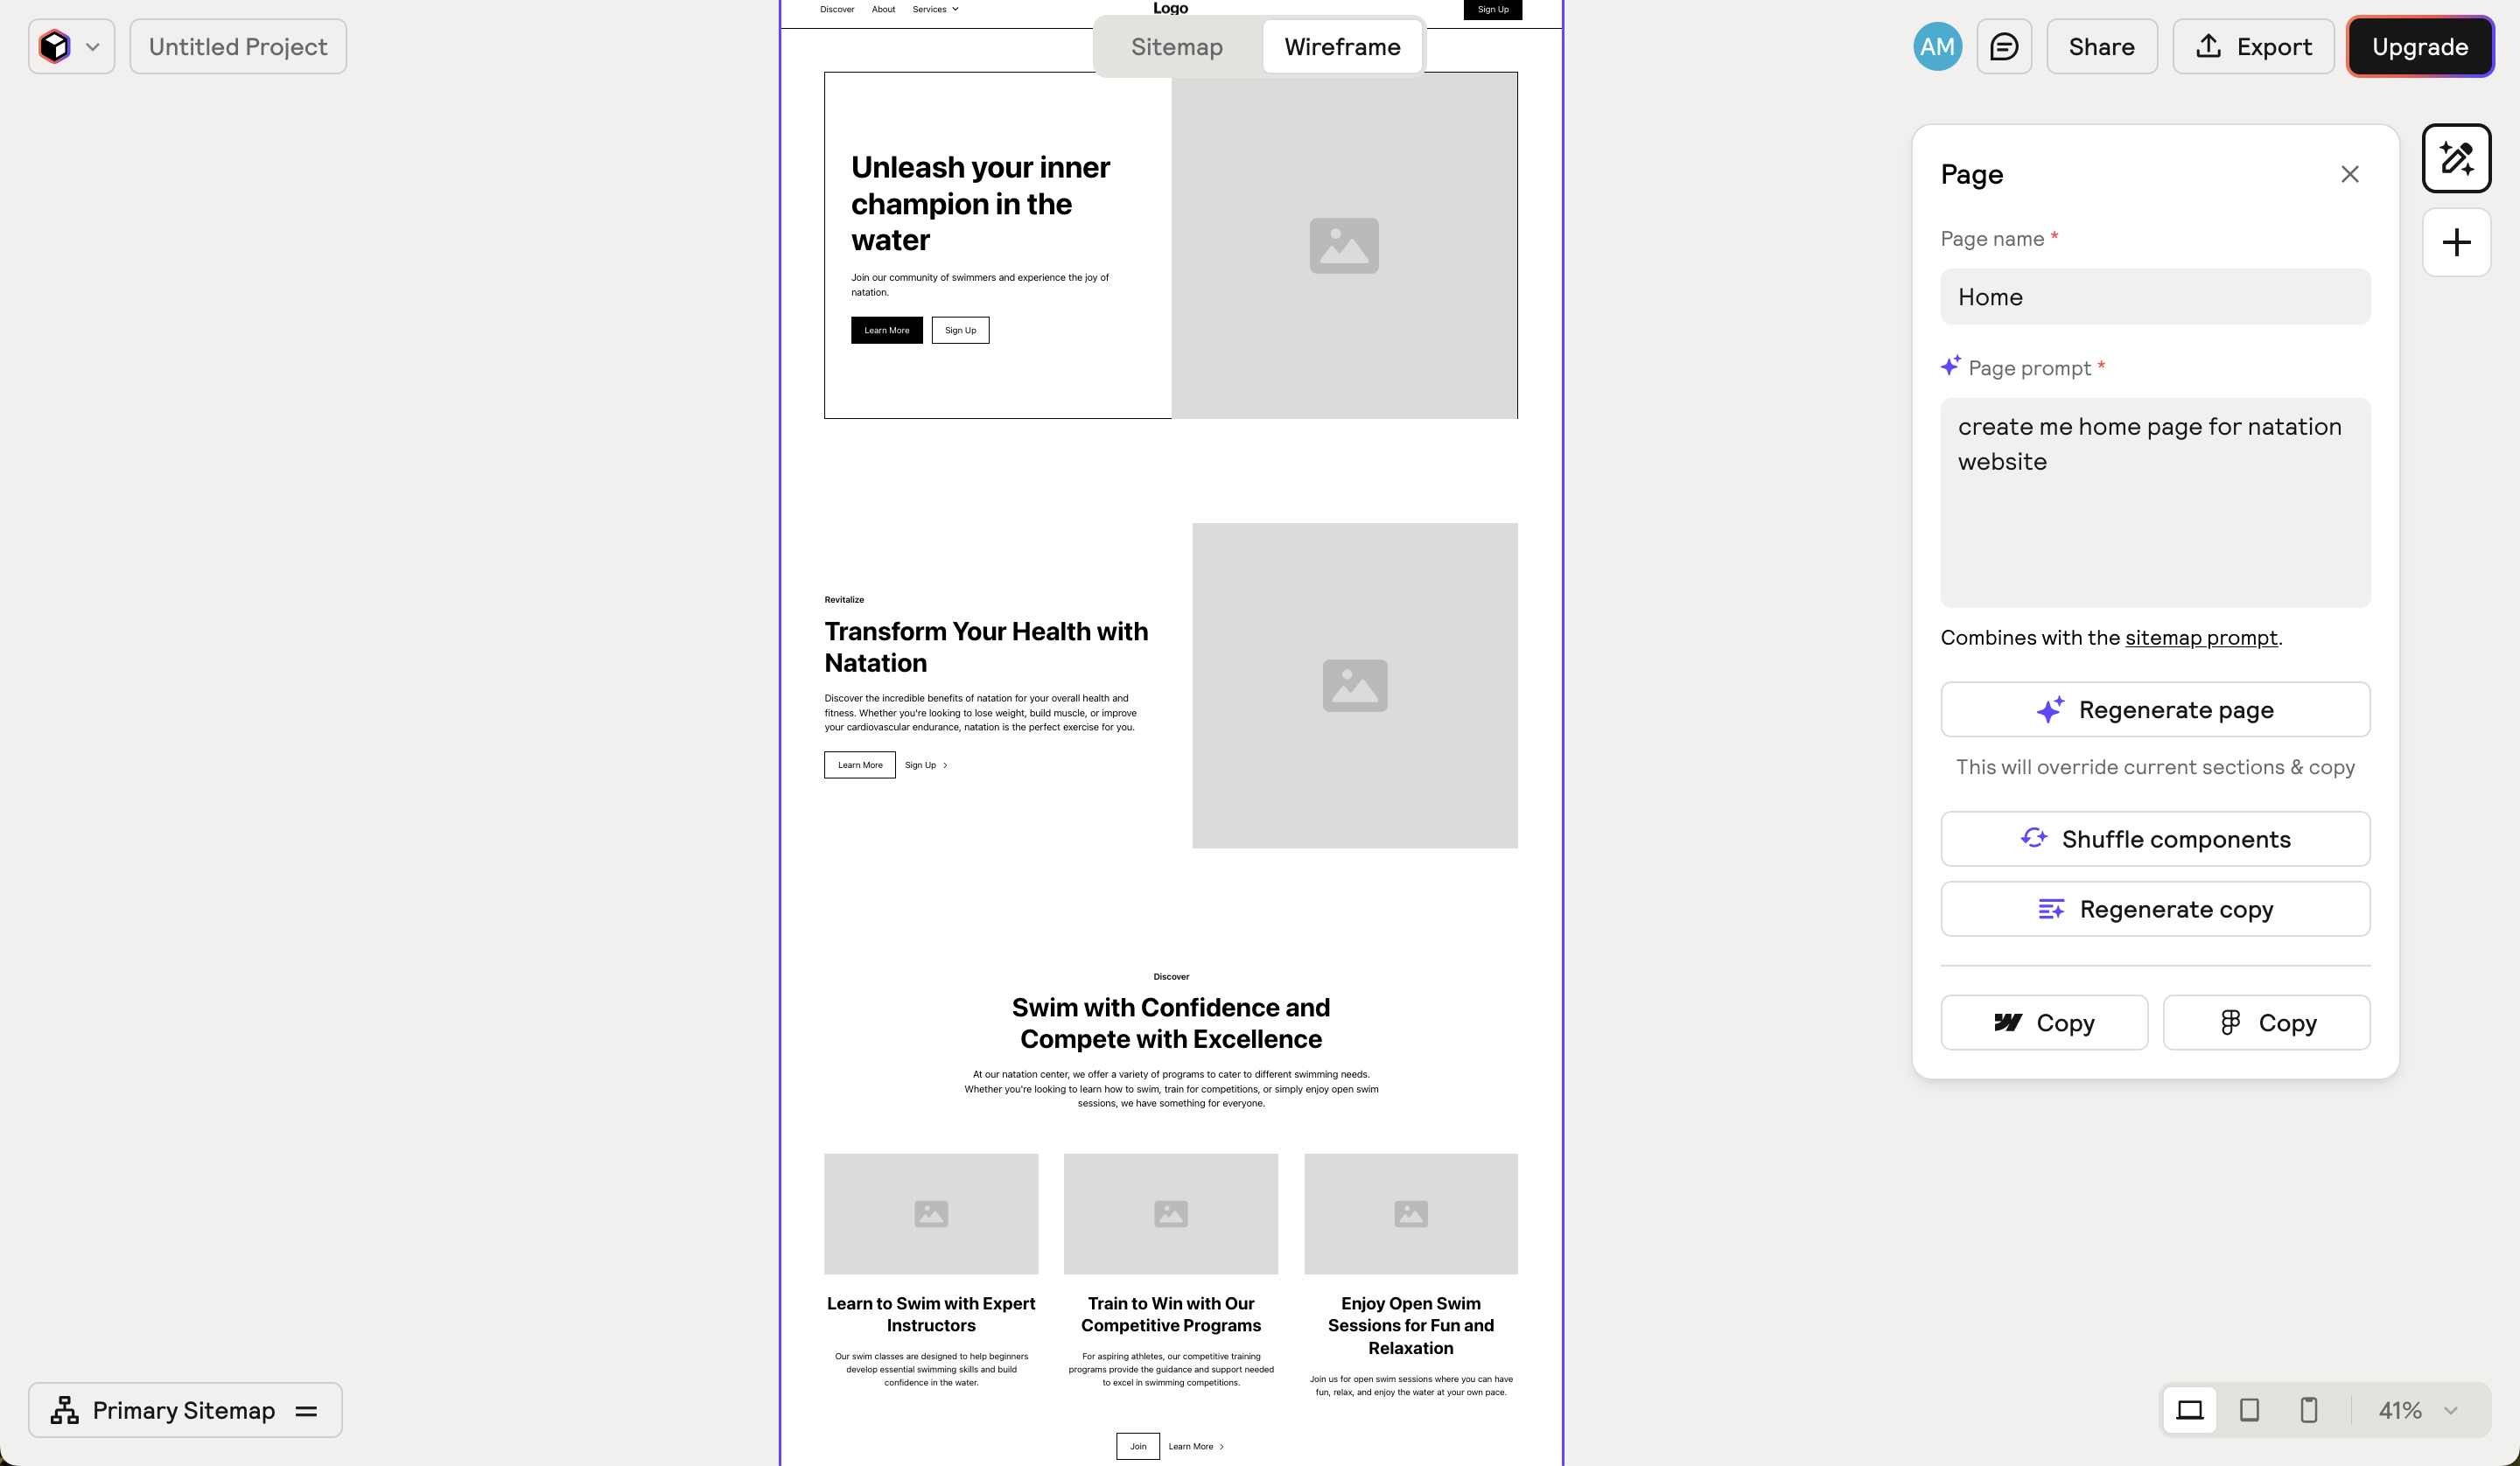
\includegraphics[width=0.8\textwidth]{Includes/Images/relume.png}
  \caption{Exemple de génération de site web sur la natation avec Relume}
  \label{fig: relume}
\end{figure} 

De plus, Relume est particulièrement efficace pour les sites classiques, comme les sites e-commerce, qui utilisent souvent des composants récurrents tels que des carrousels, des barres de navigation, des pieds de page, etc. La génération automatique de ces éléments permet de gagner un temps précieux tout en garantissant une structure cohérente et professionnelle. Relume offre également la possibilité de générer des contenus textuels en français, bien que ceux-ci soient souvent génériques.


Nous pouvons voir un exemple d'une génération de site web sur la natation avec Relume, nous pouvons voir la structure du site, les pages et les composants générés automatiquement (voir figure \ref{fig: relume}).
C'est idéal pour les projets simples, Relume se distingue par sa capacité à augmenter la productivité tout en simplifiant la gestion des projets web. Toutefois, pour des projets plus complexes nécessitant des designs et des contenus plus personnalisés, l’intervention humaine reste indispensable. 

\subsection{Webflow}
Webflow est une plateforme innovante de conception et de développement de sites web qui permet de créer des sites professionnels sans nécessiter de compétences en codage. Intégrant un éditeur visuel intuitif, Webflow permet de concevoir et de personnaliser des pages web à l'aide de fonctionnalités de glisser-déposer, tout en appliquant des styles CSS en temps réel. Les capacités avancées d'interactions et d'animations permettent de créer des expériences utilisateur engageantes, sans écrire de code complexe. De plus, Webflow offre des possibilités de low code, permettant aux développeurs d'ajouter des fonctionnalités personnalisées à travers des snippets de code et des intégrations avec d'autres outils, enrichissant ainsi l'expérience et les capacités du site. Webflow représente ainsi une solution complète et accessible alliant design esthétique et performance technique.

\subsection{DevLink}
DevLink constitue un outil de WebFlow qui facilite l'intégration des composants créés dans WebFlow à notre code (exclusivement React). Cette fonctionnalité permet d'exporter les composants créés dans WebFlow directement en code React via une simple ligne de commande. De surcroît, elle assure la synchronisation de nos composants dans notre code avec WebFlow. Ainsi, nous sommes en mesure d'importer les composants élaborés sur WebFlow dans notre code React, et de les mettre à jour automatiquement lorsque le designer effectue des modifications depuis WebFlow. 

\subsection{Contentful}
Contentful est une plateforme de gestion de contenu (CMS headless) conçue pour répondre aux besoins des développeurs. Avec son architecture flexible basée sur le cloud et son API robuste, Contentful offre une solution de gestion de contenu, les développeurs peuvent facilement intégrer Contentful à n'importe quelle technologie frontend grâce à ses API RESTful et GraphQL. Cela permet une séparation claire entre le backend et le frontend, offrant ainsi une plus grande liberté de conception et une expérience de développement plus fluide. De plus, Contentful prend en charge la collaboration en équipe avec des fonctionnalités telles que les environnements de développement, les workflows de contenu et la gestion des droits d'accès, ce qui en fait un outil incontournable pour créer des expériences web dynamiques et évolutives.

\section{Reflexion sur les difféntes possibilité d'interactions entre les outils}
Avec l'équipe nous avons réflechie sur les difféntes possiblités d'interactions.

\subsection{Possibilité n°1 - Basique}
\begin{figure}[h] 
  \centering
  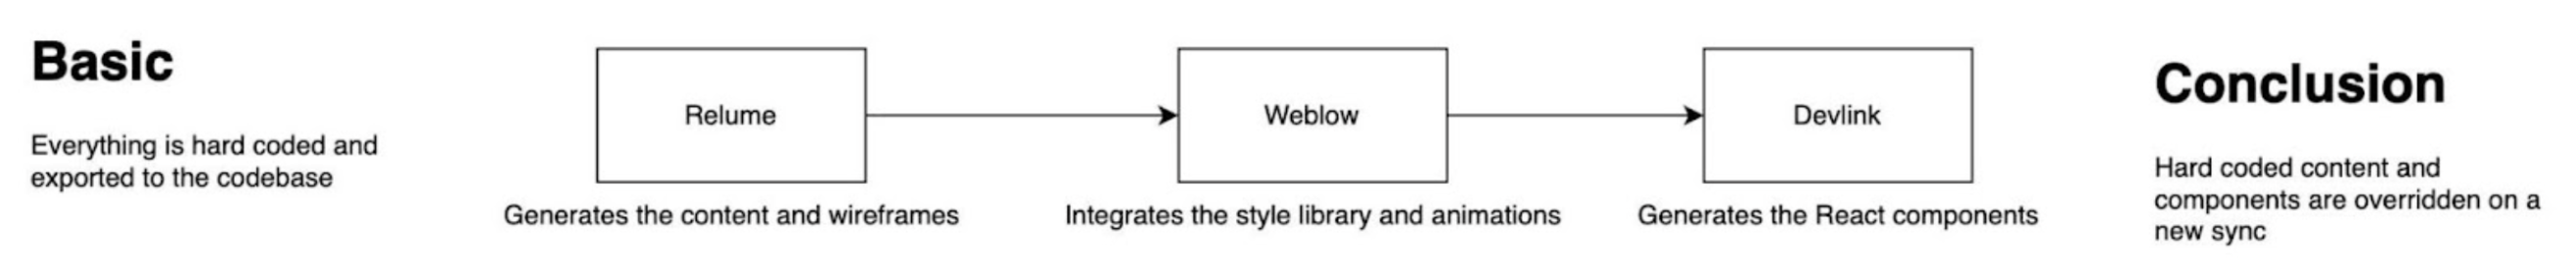
\includegraphics[width=1\textwidth]{Includes/Images/connection1.png}
  \caption{Schéma de la possibilité n°1 - Basique}
  \label{fig: Schéma de la possibilité n°1 - Basique}
\end{figure} 
La première option, la plus basique, consiste à rassembler simplement les outils (voir figure \ref{fig: Schéma de la possibilité n°1 - Basique}). Le but est de créer le site sur Relume, qui génère toute l'expérience utilisateur (UX), les wireframes, les composants et le texte. Ensuite, nous transférons tout ce que nous avons construit sur Webflow pour créer l'interface utilisateur (UI), styliser le site, ajouter des animations, etc. Enfin, avec DevLink, nous exportons tous nos composants pour les intégrer dans notre code React. Cependant, tout le texte et le contenu sont codés en dur. Si nous souhaitons modifier le texte ou les images, nous devons resynchroniser DevLink et reconstruire le site avec Next.js.

Cette méthode présente l'avantage de simplifier le processus initial de création et de design, mais elle impose des contraintes en termes de maintenance et de mises à jour de contenu. Pour chaque modification de texte ou d'image, il est nécessaire de passer par une étape de synchronisation et de reconstruction, ce qui peut être laborieux et chronophage.

\subsection{Possibilité n°2 - Avec un CMS}

Avec un CMS : L'objectif ici est de connecter Relume directement ou indirectement (via un webhook) à un CMS, afin que Relume prenne en compte le texte du CMS et l'enregistre à chaque génération. Cela permet de rendre le texte modifiable dynamiquement dans le CMS et de ne pas le perdre à chaque régénération des wireframes.

\begin{figure}[h] 
  \centering
  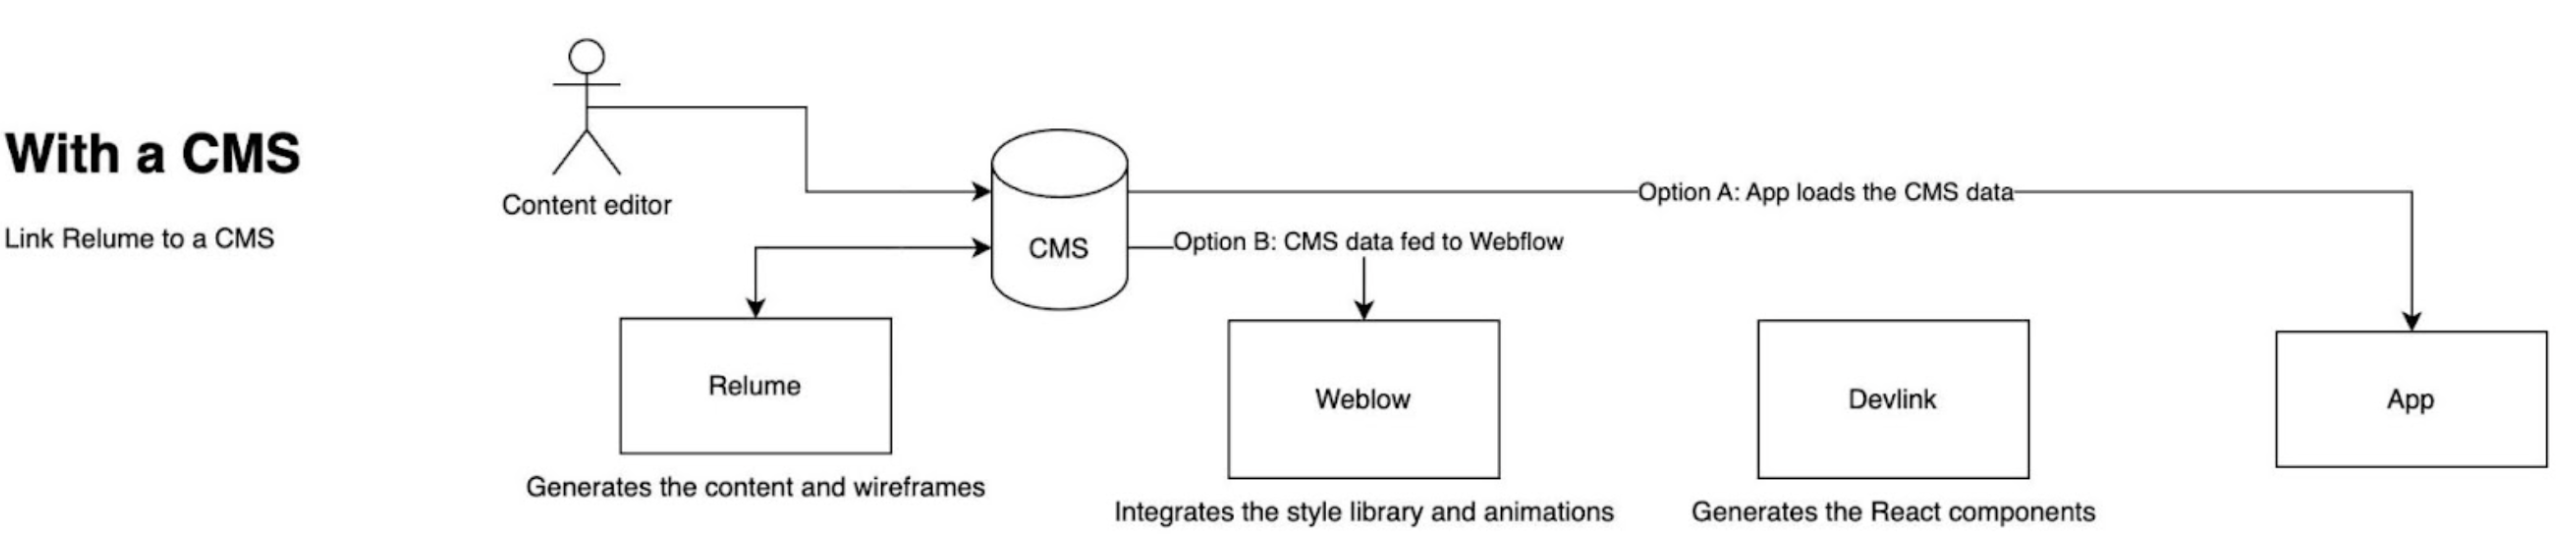
\includegraphics[width=1\textwidth]{Includes/Images/connection2.png}
  \caption{Possibilité n°2 - Avec un CMS, option A}
  \label{fig: Possibilité n°2 - Avec un CMS, option A}
\end{figure} 

Option A : Récupérer les données de la base de code React et transmettre ces données en tant que props.

\begin{figure}[h] 
  \centering
  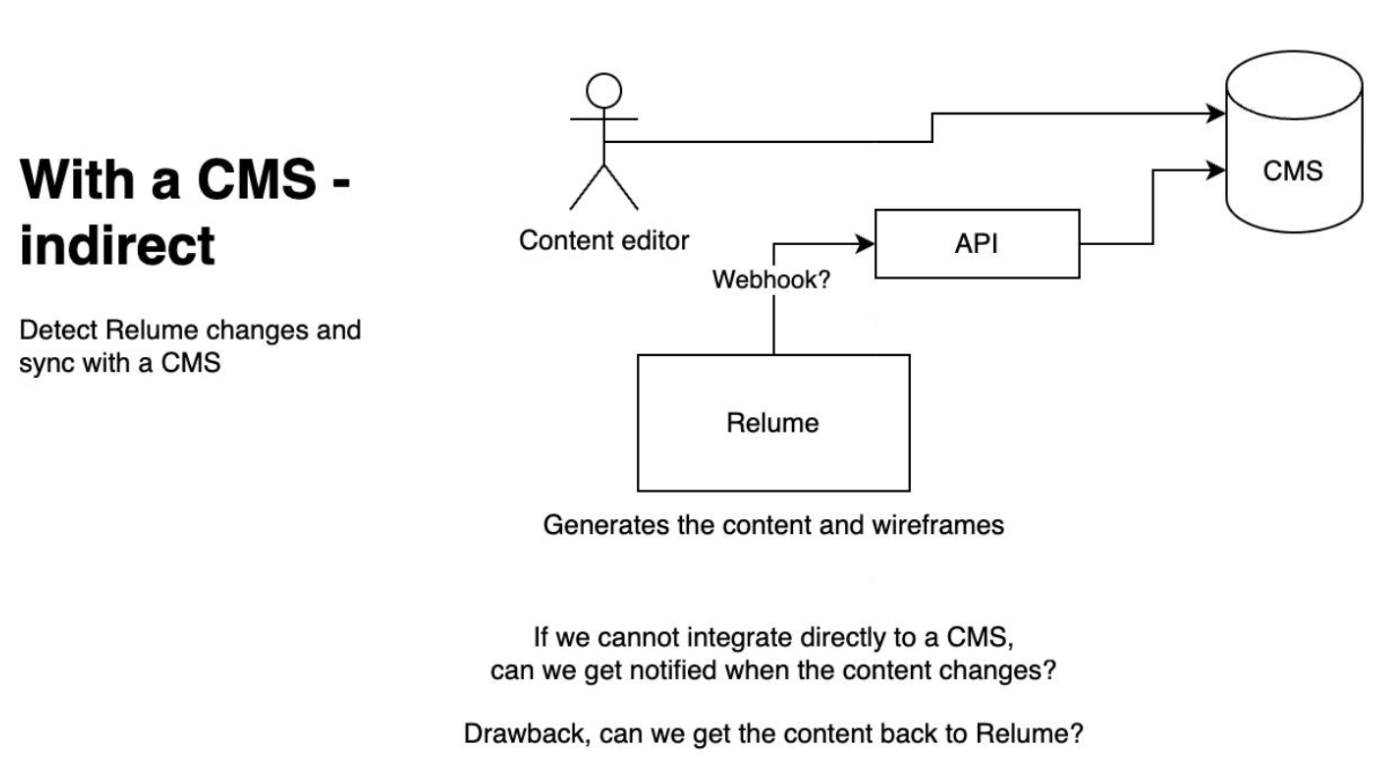
\includegraphics[width=1\textwidth]{Includes/Images/connection3.png}
  \caption{Possibilité n°2 - Avec un CMS, option B}
  \label{fig: Possibilité n°2 - Avec un CMS, option B}
\end{figure} 

Option B : Récupérer le texte et les données du CMS dans Webflow pour les exporter avec des données dynamiques. Cependant, cette méthode nécessiterait une nouvelle exportation à chaque fois qu'il y a un changement dans les informations.

Cette approche offre la flexibilité de modifier le contenu directement dans le CMS sans avoir à resynchroniser et reconstruire l'ensemble du site. Elle permet également de maintenir le contenu à jour plus facilement, bien que l'option B puisse impliquer des opérations supplémentaires lors de chaque modification des informations.